% !TEX root = main.tex

% TODO:
% REMARK:

\section{Physical Objects Reconstruction and Selection}
\label{sec:PhysObj}


	\subsection{Track}
	\label{ssec:PhysObj_track}
		%https://inspirehep.net/literature/1298029
		%https://inspirehep.net/literature/1605397

		Before reconstructing the track, it is necessary to do the $\textbf{local}$ $\textbf{reconstruction}$ which contain several terms to reconstruct the hits. There are hit reconstruction of pixel detector and strip detector, and the hit efficiency and resolution should be completely considered. To be more specific, the local reconstruction means that, in both pixel and strip detector channel, to cluster zero-suppressed signals above specified thresholds, and then to estimate the positions and uncertainty of cluster in the plane of each sensor; It is considered that the probability of finding a cluster in silicon sensor which is the record of s charged particle -- which is hit efficiency exactly; The hit resolution is to study difference between expected and measured hit positions which is called residuals. The expected one is gotten by fitted track.

		The tracking software at CMS is usually regaurded as the Combinatorial Track Finder (CTF)\cite{Billoir1989ProgressiveTR}. CTF is an adaptation of the combinatorial Kalman filter\cite{Fruhwirth:1987fm} to allow pattern recognition and track fitting to occur in the same framework.
		The track reconstructions includes four steps to proceed: (reference \cite{Chatrchyan:2014fea})

		\begin{itemize}
			\item $\textbf{Seed generation}$ : The seed defines the starting estimate of the parameters(and their uncertainty) of trajectory. That is, by only few hits, the process provide initial track candidates found. Also, the seeds are required to satisfy certain weak restrictions, for instance, minimum $p_T$.
			\item $\textbf{Track finding}$ : Based on Kalman filter, it invatigate from the seed trajectory which are gotten from seed generation along the expected flight path of charge particle. Then the purpose is to search for other probable candidates of track.
			\item $\textbf{Track fitting}$ : track fitting is a kind of module. In this stage, it yields a set of hits and an estimate of parameters of track. Because the availibility of informations should be at the final hit of the trajectory and some constraints of estimate would make bias, it has to be refitted with Kalman filter and smoother on trajectory.
			\item $\textbf{Track selection}$ : The track selection set some criteria and selected condtion to extract wanted tracks. In other words, it reduces the fake-track(which is defined as the reconstructed track which is not associated with charged particle) presenting rate through some quality requirements.
		\label{PhysObj:itm:track_reco}
		\end{itemize}

	\subsection{Vertex}
	\label{ssec:PhysObj_vertex}

		% https://iopscience.iop.org/article/10.1088/1742-6596/110/9/092009/pdf
		The classification of vertex are roughly to be $\textbf{Primary}$ $\textbf{Vertex(PV)}$ and $\textbf{Secondary}$ $\textbf{Vertex(SV)}$. The primary vertex is reconstructed proton-proton collision and expected to be detected numerous associated tracks; The secondary vertices are the points where some particles decay when propagating. In this section, we put the emphasis on the primary vertex.

		There are many proton-proton interaction vertices which are exactly PVs in each event including signal vertex(whose interaction we have interests in) and other vertices from pileup collisions(section.\ref{ssec:PhysObj_pu}). The work of finding position of primary vertex is highly related to reconstructed tracks. The three steps of reconstructing primary verex is shown below:

		\begin{itemize}
			\item $\textbf{Tracks selection}$ : To choose the tracks which are produced in the primary interaction region and also consistent, there are some requirements. It is set on the significance of the transverse impact parameter, the number of pixel/strip hits related to one track, and $\chi^2$ value which is normalized from fitting to the trajectory. However, there is no tracks' $p_T$ selection because of the confirmation of high econstruction efficiency.
			\item $\textbf{Tracks clustering}$ : Tracks clustering is now using $\textbf{Deterministic}$ $\textbf{Annealing(DA)}$\cite{726788} algorithm which can find global minimum under multi-dimention space(multi- degrees of freedom). By the ability, it can cluster the tracks which appears to originate from the same interaction vertex. The algoeithm detail can be probed in \cite{Chatrchyan:2014fea} and \cite{726788}.
			\item $\textbf{Track fitting}$ : By vertex's associated tracks, the vertex position would be fitted. After identifying candidates vertices by DA algorithm, the candidates vertices would be fitted by using $\textbf{adaptive vertex fitter}$\cite{Fruhwirth:2007hz}. Then the best estimation of vertices' parameter would be got. For example, x, y and z position, covariance matrix, number of D.o.F(degrees of freedom) for the vertex, and also weights of the tracks which account for the vertex, etc.
		\label{PhysObj:itm:track_reco}
		\end{itemize}

	\subsection{Pileup Issue}
	\label{ssec:PhysObj_pu}{}

		% https://cms.cern/news/reconstructing-multitude-particle-tracks-within-cms
		Because of the high luminosity of pp collision in CMS, there are more than one pp collision occuring in every time when the the bunches cross one another. The multiple collision in one crossing event is called $\textbf{pile-up(pileup)}$. In the present, the LHC is operating at an instantaneous luminosity of $0.7\times10^{34} cm^{-2}s^{-1}$, and the proton bunches cross inside CMS every 50 ns, so there are more proton in one bunch and showing high pileup. Also, the high granularity and efficiency of CMS Tracker make them distinguish the many tracks in an event. The pileup image is shown below(Fig.\ref{PhysObj:fig:pileup_img}). There are more information in the reference \cite{Pileup_page}.

		% https://cms.cern/news/reconstructing-multitude-particle-tracks-within-cms
		\begin{figure}[H]
		\centering{}
	    	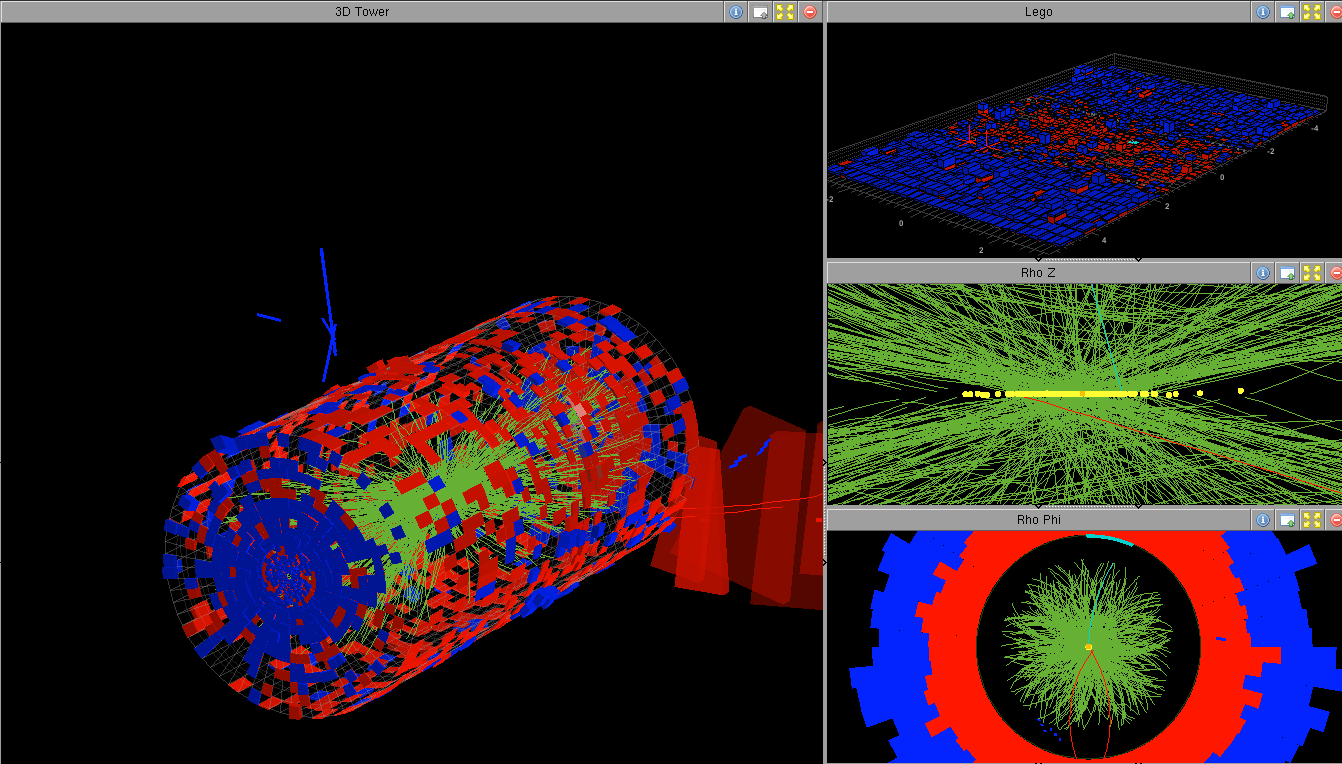
\includegraphics[width=0.85\textwidth]{Figures/PhysObj/pileup_image.png}\\
		\caption{78 reconstructed vertices in one crossing from high pileup run (3D, lego, on Pho-z plane, on Rho-Phi plane) \cite{Pileup_page}}
		\label{PhysObj:fig:pileup_img}
		\end{figure}
		\FloatBarrier



	\subsection{Lepton}
	\label{ssec:PhysObj_lep}

		The selected lepton in the analysis is required to obey the criteria of one passed $\emph{selected lepton}$ and zero $\emph{veto lepton}$ passed. The veto criteria means that there would be no lepton passing the veto criteria except the selected one. In other words, the veto criteria can filter the physical objects which are lepton-like but not really like after reconstructed from particle level to detector level. The selected criteria corresponds to tight lepton's criteria, and veto criteria follows loose lepton's criteria:

		\subsubsection{Muon}
		\label{sssec:PhysObj_MuonReco}

			To reconstruct the muons, there are some procedure should be go through. The first is about the $"\textbf{hit}"$ and segment reconstruction. The $"$hits$"$ are the electric signal produced on wires and strips when muons and other charged particles transversed. The hits reconstruction in different part of detector have different algorithm for reconstructing. Hits in DT(\ref{ssec:muon_detector}) estimate the distance between the wire and the interaction point of muon and the plane in layers. With a $\textbf{time-to-digital}$ $\textbf{converter}$$\textbf{(TDC)}$ registering their arrival time $T_{TDC}$, a time pedestal $T_{ped}$, and the drift velocity $v$, the position of DT hits are then reconstructed by the formula:

			\begin{equation}
			position = (T_{TDC} - T_{ped}) \times v
			\label{eq:MuReco_1}
			\end{equation}
			\FloatBarrier

			Hits which are reconstructed in CSC layers combine information from anode wires and cathode strips to measure traversing muon's position; Also, the hits in RPC layers are the product of hit strips clustering. It is necessary that adjacent strips are clustered to reconstruct one hit because the charge of muons which is ionized could be distributed on not just one strip; With multi-layers structure of DT and CSC, their reconstructed hits are built as $\textbf{segment}$.

			Secondly, the tracks are reconstructed independently and eventually used as input for muon track reconstruction. There are steps to reconstruct the muon tracks:

			\begin{itemize}
				\item $\textbf{Standalone-muon tracks}$ : By using Kalman-filter technique\cite{Fruhwirth:1987fm} and information from subdetectors(DT,CSC,PRC), standalon-muon track is built. The reconstruction starts from seeds which are composed of sets of DT/CSC segments.
				\item $\textbf{Tracker muon tracks}$ : They are built $"$inside-out$"$ from tracker tracks to the muon system(segments). 
				\item $\textbf{Global muon tracks}$ : They are built $"$outside-in$"$ by matching the reconstructed standalone-muon tracks to the tracker tracks.
			\label{PhysObj:itm:muon_track_reco}
			\end{itemize}

			Muons are often reconstructed as a global muons track or a tracker muons track or almost as both. It is merged to the muon canndidate that the global muon and the tracker muon share the same tracker tracks.

			The third one is to identify the muon.($\textbf{Muon Identification}$$\textbf{(Muon ID)}$) Sets of variables are studied and developed to be selection criteria, for example, the $\chi^2$ track fit, the $\#$ of hits in one track...,etc.(Most are based on information in muon reconstruction) The muon ID used in the analysis are listed below:

			\begin{itemize}
				\item $\textbf{Loose muon ID}$ : A muon is selected by PF algorithm that is either a global or a tracker muon.
				\item $\textbf{Tight muon ID}$ : The muon must be simultaneously global and tracker muon after reconstructed. The global muon fit must have goodness of fit test() with $\chi^2/d.o.f < 10$ and at least have one hit from muon chambers. A tight muon also corresponds to primary vertex compatibly, and has longitudinal impact parameter |dZ|<0.5cm and transverse impact parameter |dXY|<0.2cm.
			\label{PhysObj:itm:muon_ID}
			\end{itemize}

			The forth is to detemine the momentum of muons by the tune-P algorithm\cite{collaboration_2012}. The algorithm select one of the measuring $p_T$ results by refitting. The decision is made based on level of goodness-of-fit and to reduce the tail on the events number on $p_T$ spectrum because of poor quality fits. There are $\textbf{Inner-track}$ $\textbf{fit}$, $\textbf{Tracker}$$\textbf{-Plus}$$\textbf{-First}$$\textbf{-Muon}$$\textbf{-Station}$ $\textbf{fit}$, $\textbf{Picky}$ $\textbf{fit}$, and $\textbf{Dynamic-Truncation}$ $\textbf{fit}$:

			\begin{itemize}
				\item $\textbf{Inner-Track fit}$ : Using only inner trackers' information, appropriate for low $p_T$ range.
				\item $\textbf{Tracker-Plus-First-Muon-Station fit}$ : Starting with the global muon track, from inner tracker information and hits contained by innermost muon station(which has the best performance on momentum in the muon system), it perform the refits.
				\item $\textbf{Picky fit}$ : Starting with the global muon track, it does the refits only with hits which are compatible with the inferred trajectory.
				\item $\textbf{Dynamic-Truncation fit}$ : The algorithm refits from innermost stations outward to the outermost one. If there is no compatible hit found in 2 consecutive muon stations, it stops.
			\label{PhysObj:itm:muon_p_reco}
			\end{itemize}

			Last, muons' isolation can help distinguish prompt muons from those casued by weak decays from jets. A given muon commonly uses its $p_T$ which is summed up from the energy in the geometry cone($\Delta R = \sqrt{(\Delta \eta)^2 + (\Delta \phi)^2}$) surrounding the muon. The first choice of energy addition is summing the reconstructed tracks, and the other is to use neutral particles and charged hadrons from PF isolation.

			%\cite{Sirunyan:2018fpa} %main
			%\cite{Chatrchyan:2012xi}

			Through the complete procedure, the muons could be reconstructed. All the information and detail in section.\ref{sssec:PhysObj_MuonReco} are from ref.\cite{Sirunyan:2018fpa}. The muons passing the particle flow reconstruction should pass the selections in this analysis, and they are listed below:

			\begin{itemize}
				\item $\textbf{Selected muon criteria}$ : 
					\begin{itemize}
						\item $p_T$ > 30 GeV
						\item |$\eta$| < 2.4
						\item Pass muon ID with tight working point from Muon POG\cite{muon_POG}(\ref{PhysObj:itm:muon_ID})
						\item PF-based combined relative isolation value < 0.15 from Muon POG\cite{muon_POG}
					\end{itemize}
				\item $\textbf{Veto muon criteria}$ : 
					\begin{itemize}
						\item $p_T$ > 15 GeV
						\item |$\eta$| < 2.4
						\item Pass muon ID with loose working point from Muon POG\cite{muon_POG}(\ref{PhysObj:itm:muon_ID})
						\item PF-based combined relative isolation value < 0.25 from Muon POG\cite{muon_POG}
					\end{itemize}
			\label{PhysObj:itm:muon_selection}
			\end{itemize}
			
		\subsubsection{Electron}
		\label{sssec:PhysObj_ElectronReco}

			To reconstruct electrons, The approach is to cluster the energy in ECAL and then assocciate them to the reconstructed tracks. The global particle-flow(PF) algorithm and a standalone approach are used. The first step is to cluster electron energy in ECAL. Though the energy of electron spreads and losed little portion before reacching ECAL's crystal, the effects of inducing radiating photon from electrons are large. That is to say, in CMS detector the bending motion of electron caused by magnetic fields is accelerating motion, so the electrons often radiate photons that mainly spreads along $\phi$ direction.(The spreads on $\eta$ direction is usually neglected except for low $p_T$ case) Therefore, the collection of induced photons' energy and clustering them is required. There are two clustering algorihtm used -- $\textbf{hybrid}$ $\textbf{algorithm}$ for the barrel and $\textbf{multi-5}$$\times$$\textbf{5}$ $\textbf{algorithm}$ for the endcaps. In both algorithm, the clusters assemble and have the requirement of energy exceeding some threshold, then they would be called $\textbf{superclusters(SC)}$.

			The following is to reconstruct the electron tracks by the standard Kalman filter method in tracker. Because of the reduced hit-collection efficiency from electrons' large radiative losses and shortage of estimation of track parameters, a dedicated tracking procedure is adopted. There are twon primary parts of the procedure -- $\textbf{seeding}$ and $\textbf{tracking}$. Seeding is to find two orr three hits in the tracker from which the reconstructed track initiate. There are also two complementary algorithm for greater reconstrruction efficiency -- $\textbf{ECAL-based}$ $\textbf{seeding}$ and $\textbf{tracker-based}$ $\textbf{seeding}$. The ECAL-based algorithm helps estimating the electrrons' trajectory in the first layers of the tracker, and the method begins with the position and SC energy. The tracker-based seeding is dependent on the reconstructed tracks and extending to the SC and ECAL. The seeding steps usually uses the standard KF algorithm directly. However, if the potential presence of bremsstrahlung significantly show, it is then adopted that the $\textbf{Gaussian}$ $\textbf{sum}$ $\textbf{filter}$$\textbf{(GSF)}$ method. Then the inforrmation from KF method, GSF method, ECAL, and tracker would be poured into multi-variate analysis(MVA) to get the chosen electron seeds. After electrons' seeds are selected, they are used to initiate electron track building. The tracking is from the initial seed and then fitted with KF or GSF method. The constraints are included to reduce the increasing trajectory candidates from fitting results of increasing layers. As a result, the electron track is reconstructed.Also, the electron particle-flow clustering is driven by GSF tracks, and it is independent to the seeded way.

			The electron charge is estimated by the bremsstrahlung followed by photon conversions. Because the remsstrahlung photons convert and lead to complex hit-patterns, the fitting of electron track would penetrated from the wrongly contributions from this conversion. The solving is about the sign of the GSF track curvature, and it has improvements from combination of 2 charge estimation. The first is about match between the associated KF track and a GSF track, and the second one is evaluation about SC position($\phi$ difference of vector joining the beam spot, SC and the first hit of the electron GSF track). Last, the electrons' momentum is evaluated by combination of the tracker and ECAL information. It is classified with their bremsstrahlung pattern for electrons, because the electrons' sensitivity to the emission and the conversion of photons could provide the better electron momentum measurements.

			The details of electrons' reconstruction could be checked in ref.\cite{2015_el_reco}.

			The electrons passing the particle flow reconstruction should pass the selections in this analysis, and they are listed below:

			\begin{itemize}
				\item $\textbf{Selected Electron criteria}$ : 
					\begin{itemize}
						\item $p_T$ > 38 GeV
						\item |$\eta$| < 2.4 $\&$ $\notin$ [1.4442, 1.5660]
						\item Pass electron ID with tight working point from EGamma POG\cite{egamma_POG}()
						\item impact parameter cut from EGamma POG\cite{egamma_POG}
					\end{itemize}
				\item $\textbf{Veto Electron criteria}$ : 
					\begin{itemize}
						\item $p_T$ > 15 GeV
						\item |$\eta$| < 2.4 $\&$ $\notin$ [1.4442, 1.5660]
						\item Pass electron ID with loose working point from EGamma POG\cite{egamma_POG}()
						\item impact parameter cut from EGamma POG\cite{egamma_POG}
					\end{itemize}
			\label{PhysObj:itm:electron_selection}
			\end{itemize}

	\subsection{Missing Transverse Energy(MET)}
	\label{ssec:PhysObj_met}
		The $\textbf{missing}$ $\textbf{transverse}$ $\textbf{energy}$$\textbf{(MET)}$ is a physical objects about invisible particles in CMS detector, for example, neutrino. Because of the momentum conservation before and after the collision, the kinematics of invisible stuffs would be inferred. The approach to get the missing energy is summing up the visible final physical object's momentum with a minus sign added. The x/y-direction's initial momentum($p_x$,$p_y$) are known being zero respectively, but initial momentum z-component($p_z$) is unknown because of the pileup bunches and messy collision. Therefore, the practical part of missing energy to be calculated is the transverse part(x-y plane) of momentum -- the missing transverse energy. The measurement of MET is shown below:

		\begin{equation}
		missing\;E_T = - \sum_{i}^{} \vec{p}_{T,i} \;, \; i\;for\;visible\;final\;objects
		\label{eq:MET}
		\end{equation}
		\FloatBarrier
		

	\subsection{Jet}
	\label{ssec:PhysObj_jet}

		% Jet reco : Atkin_2015_J._Phys.__Conf._Ser._645_012008
		% anti-k algo : M. Cacciari, G. P. Salam, and G. Soyez, “The anti-k(t) jet clustering algorithm”, JHEP 04, 063 (2008)

		Jet is a type of physical object in high energy collider/detector physics. There are cluster of stable particles after collision, then fragmentating and hadronizing to be a jet. In the process, the strong interaction quarks and gluons cause the showering of these particles. And there is also some algorithm to reconstruct the showering to be an object -- jet, by some calormeter's and tracker's information.
		The used algorithm is anti-k algorithm to reconstruct all jets. The algorithm summarization is shown follow. First, there is a list of particles which are candidates of jets' member, they are called protojet. Secondly, for any i-th protojet, we find the minimum $d_{ij}$ and minimum $d_{iB}$ in the list. The $d_{ij}$ and $d_{iB}$ are defined below:

		\begin{equation}
		\begin{split}
		d_{ij} = min(P_{Ti}^{2p}, P_{Tj}^{2p}) \frac{\Delta_{ij}^2}{R^2}\\
		, \Delta_{ij} = \sqrt{ (\eta_i - \eta_j)^2 + (\phi_i - \phi_j)^2 }\\
		d_{iB} = P_{Ti}^{2p}
		\end{split}
		\label{eq:jet_reco_algo}
		\end{equation}
		\FloatBarrier

		In the definition, $P_{T}$, $\eta$ and $\phi$ individually means the transverse momentum, rapidity and azimuth of protojet. Also, the $\Delta_{ij}$ means the distance between i-th protojet and j-th protojet under $\eta$-$\phi$ space. Besides the radius parameter R, the p is the important parameter which decide the power of energy scale. The following step is to compare the minimum $d_{ij}$ and minimum $d_{iB}$, if the min-$d_{ij}$ is smaller than min-$d_{iB}$, then remove i-th and j-th protjets out of the list, and combine the i-th and j-th protojets into a new protojet and add in the original protojet list; if the min-$d_{ij}$ is larger than min-$d_{iB}$, then the i-th protojet is considered as a jet and remove it from the list of portojets. And then, choose the new i-th protojet and do the previous comparison and assignment again and again. The algorithm stops as long as the list of protojets is empty. The illustration example of algorithm is shown below(Fig.\ref{PhysObj:fig:jet_algo}). Furthermore, in CMS we commonly apply R by 0.4 as the AK4 jet, which is also used in the analysis. If the parameter $p=1$, it is called inclusive $k_{t}$ algorithm; and if $p=0$, Cambridge/Aachen algorithm; and if $p=-1$, anti-$k_{t}$ jet-clustering algorithm. For CMS, because of the high pileup property, it used to use $p=-1$ case -- anti-$k_{t}$ algorithm to construct jets. The behavior of different jet-reconstruction algorithm under $\eta$-$\phi$ space are shown in Fig.\ref{PhysObj:fig:3type_jetreco}. The informations are from \cite{Atkin_2015} and \cite{Cacciari_2008}.

		\begin{figure}[H]
		\centering{}
	    	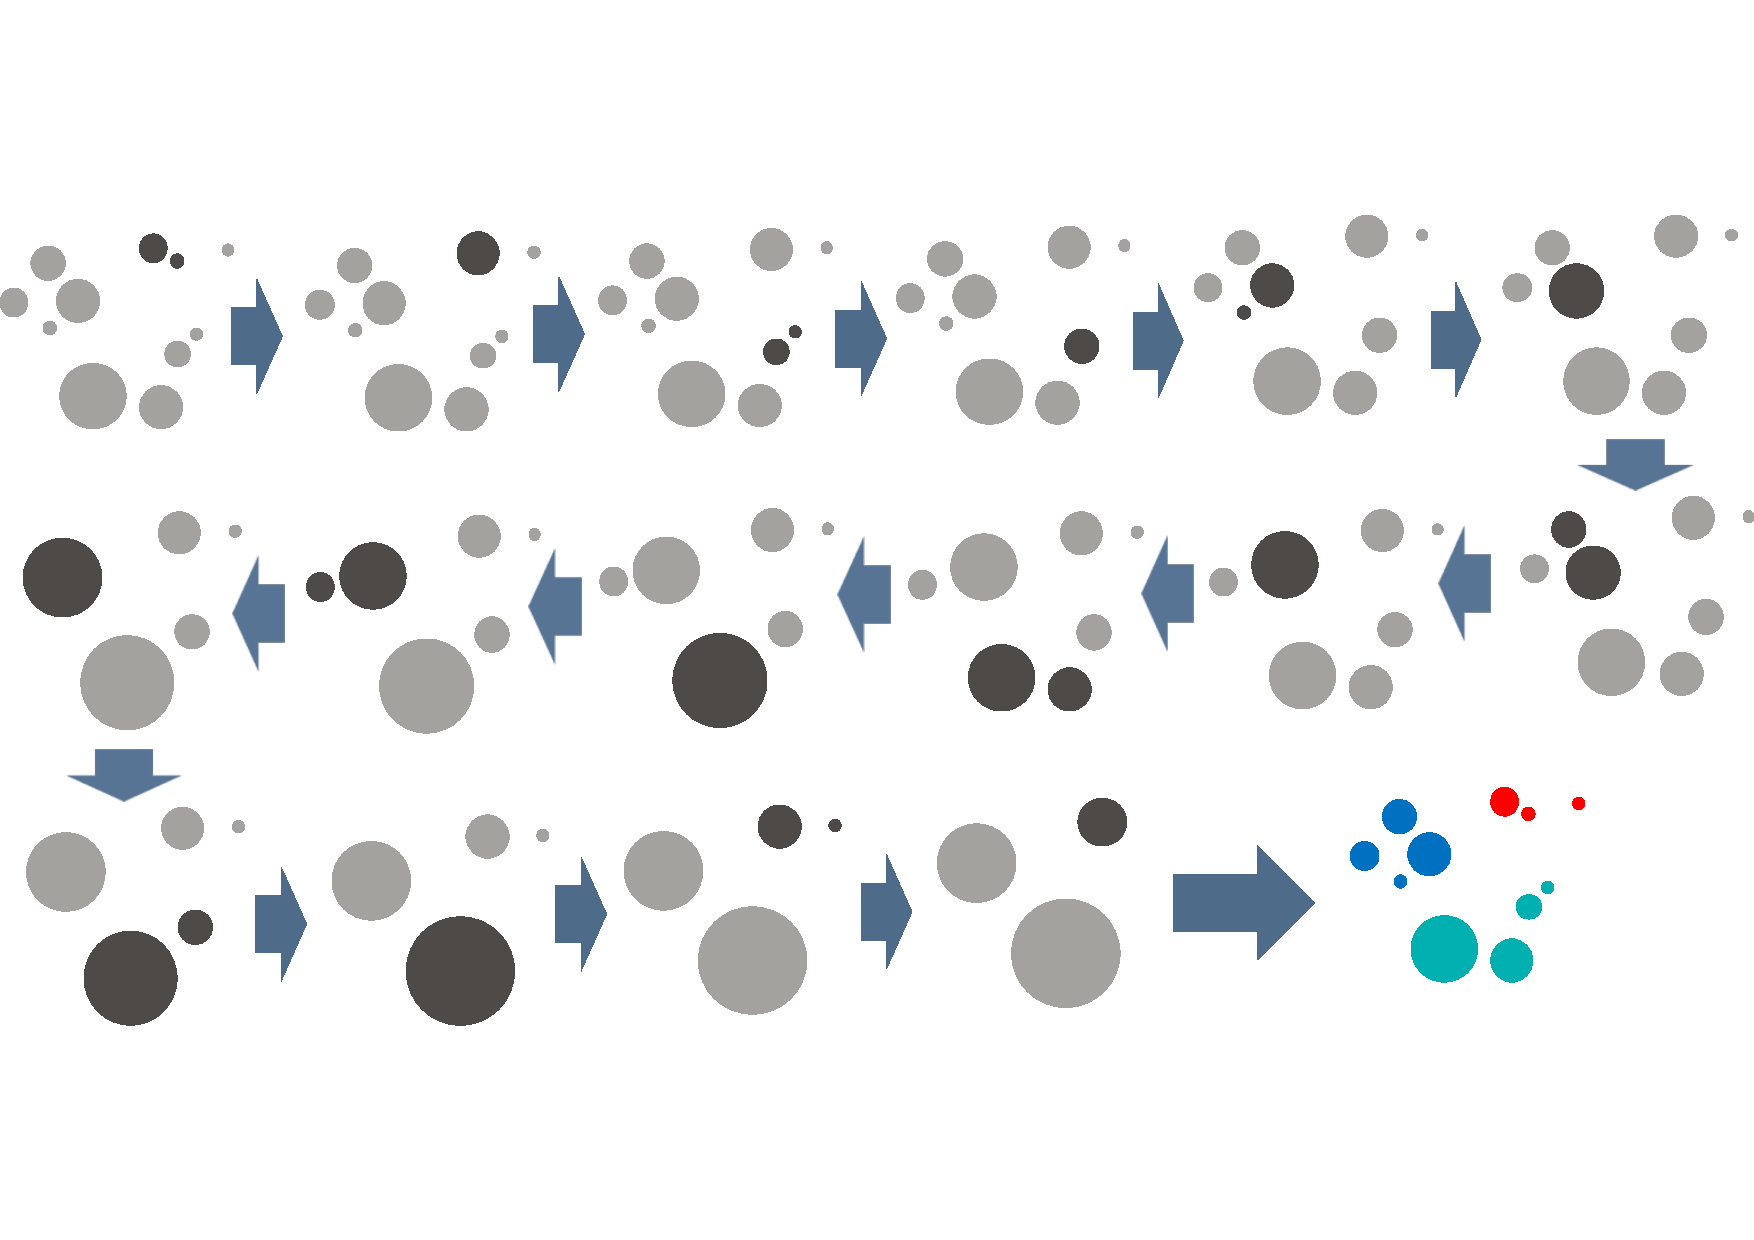
\includegraphics[width=0.85\textwidth]{Figures/PhysObj/jet_algo.pdf}\\
		\caption{Illustration diagram about an example of constructing protojets to jets}
		\label{PhysObj:fig:jet_algo}
		\end{figure}
		\FloatBarrier

		\begin{figure}[H]
		\centering{}
	    	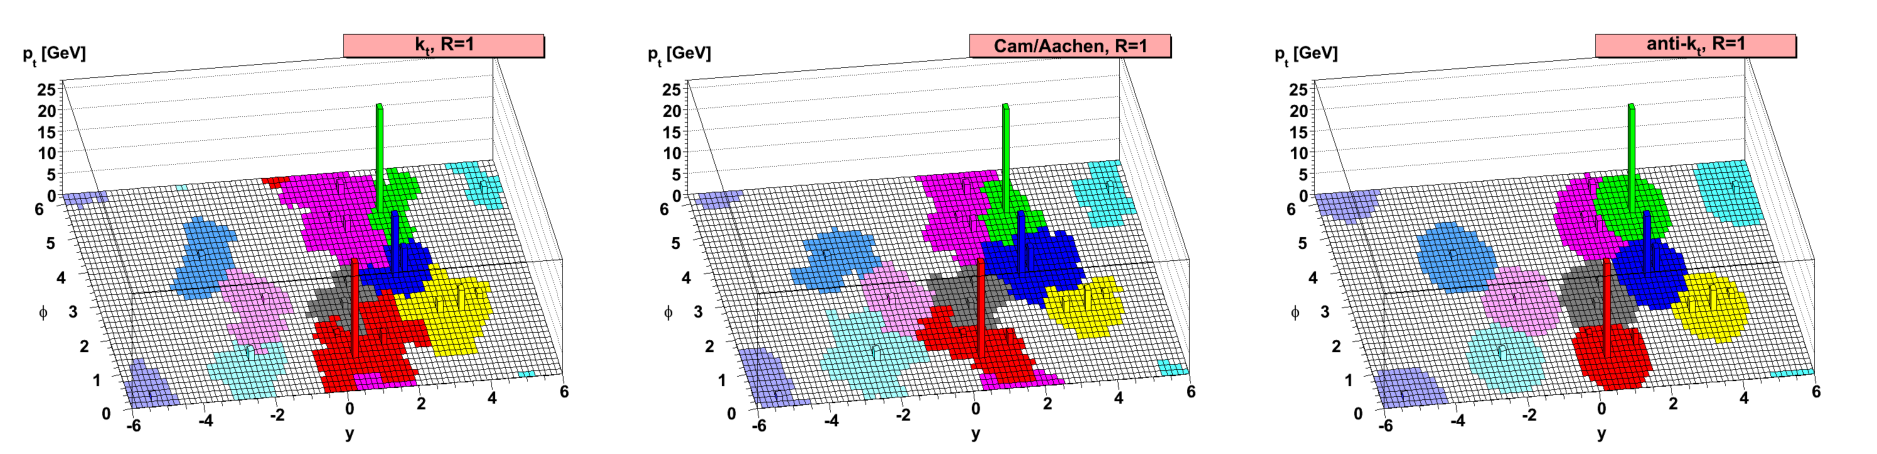
\includegraphics[width=0.85\textwidth]{Figures/PhysObj/3type_jetreco.pdf}\\
		\caption{behavior difference between $k_t$/CA/anti-$k_t$ algorithm \cite{Atkin_2015}}
		\label{PhysObj:fig:3type_jetreco}
		\end{figure}
		\FloatBarrier

		When reconstructing jets, the energy of jets have to be calibrated by jets' $P_T$ and $\eta$. It is named $\textbf{Jet}$ $\textbf{Energy}$ $\textbf{Calibration}$$\textbf{(Correction)}$$\textbf{(JEC)}$\cite{collaboration_2011_JEC}. The correction applies a multiplicative factor $C_{cor}$ to the four-monmentum of raw jets. The factor $C_{cor}$ is a product of offset correction, MC calibration factor, absolute energy scale and residuals calibrations. All of the four ingredients are partially relative to jets' $p_T$ and $\eta$.(Eq.\ref{eq:JEC_1})

		\begin{equation}
		\begin{split}
		p_{\mu}^{cor} = C_{cor} \cdot p_{\mu}^{raw} \; \; \; \; \; \; \; \; \; \; \; \; \; \; \; \; \; \; \; \; \; \; \; \; \; \; \; \; \; \; \; \; \; \; \; \; \; \; \; \; \; \; \; \; \; \; \; \; \\
		C_{cor} = C_{offset}(p_T^{raw}) \cdot C_{MC}(p'_T,\eta) \cdot C_{abs}(p''_T) \cdot C_{rel}(\eta)
		\end{split}
		\label{eq:JEC_1}
		\end{equation}
		\FloatBarrier

		In addition to the Jet energy calibrattion, there is also $\textbf{Jet}$ $\textbf{Energy}$ $\textbf{Resolution}$$\textbf{(JER)}$ considered\cite{JER_twiki}. The issue come from that the jet energy resolution in data is worse than in MC simulation, so we need to correct the resolution in MC with scaling and smearing method to closely describe the data. For a jet, if a well-matched particle-level jet is present(Eq.\ref{eq:JER_0} are the requirements for the matching), the scaling method is adopted. Scaling method scale the four-momentum of jets with a factor $c_{JER}$(Eq.\ref{eq:JER_1}):

		\begin{equation}
		\Delta R < R_{cone}/2, \; \; \; |p_T-p_T^{ptcl}| < 3 \sigma_{JER} \cdot p_T
		\label{eq:JER_0}
		\end{equation}
		\FloatBarrier

		where the $R_{cone}$ is the cone size parameter, in the analysis with AK4 jet, the $R_{cone}$ is 0.4. Also, the $\sigma_{JER}$ is the width which is the resolution measured from MC.

		\begin{equation}
		c_{JER} = 1 + (s_{JER} - 1)\frac{p_T-p_T^{ptcl}}{p_T}
		\label{eq:JER_1}
		\end{equation}
		\FloatBarrier

		The $p_T$ is the transverse momentum of jet, and $p_T^{ptcl}$ is the transverse momentum of the corresponding jet clustered from generator-level particles. $s_{JER}$ is the data-to-MC core resolution scale factor. If the $c_{JER}$ is measured negative, it is set to be zero, that is to say, the factor $c_{JER}$ truncated at zero; In the other case that doesn't require the presence of well-match jet, it is set to adopt the smearing method(Eq.\ref{eq:JER_2}):

		\begin{equation}
		c_{JER} = 1 + N(0,\sigma_{JER})\sqrt{max(s_{JER}^2-1,0)}
		\label{eq:JER_2}
		\end{equation}
		\FloatBarrier

		The selected jets in the analysis comply with the criteria below:

		\begin{itemize}
		\item $p_T$ > 30GeV
		\item $|\eta|$ < 2.4
		\item $\Delta R$ < 0.4 with the selected lepton
		\item pass Jet Loose ID : \cite{JetLooseID_twiki}
		\begin{itemize}
			\item neutral hadron energy fraction < 0.99
			\item neutral EM fraction < 0.99
			\item charged hadron fraction > 0
			\item number of constituents > 1
			\item charge multiplicity > 0
			\item charged EM fraction < 0.99
		\end{itemize}
		\label{PhysObj:itm:sel_jet}
		\end{itemize}
		

		\subsubsection{b-tagged jet}
		\label{sssec:bjet}

			To precisely identify the type of original particle of jets, some algorithm are computed to be a discriminator. Instead of light-flavor(udsg), there are commonly heavy-flavor(b,c) jet discriminator using some variables to identify the properties of jets from the radiation and hadronization of b or c quarks, for example, the hadrons containing b quark's lifetime is more longer than ones with c quarks. In this analysis, b-quark discriminator is handed to pick up the b quarks decaying from t quarks. According to the long lifetime of b hadrons, this would cause displacements of a few mm to one cm for b hadrons. The displaced tracks construct the secondary vertex(SV). The illustration diagram of primary vertex and secondary vertex is shown in Fig.\ref{PhysObj:fig:PV_SV}. 

			\begin{figure}[H]
			\centering{}
		    	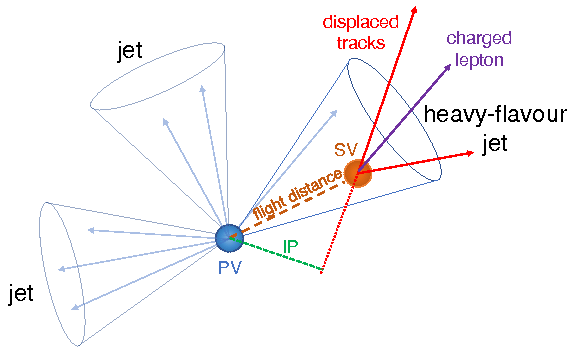
\includegraphics[width=0.85\textwidth]{Figures/PhysObj/PV_SV.png}\\
			\caption{Illustration of useful variables for b tagging \cite{CMS-BTV-16-002}}
			\label{PhysObj:fig:PV_SV}
			\end{figure}
			\FloatBarrier

			The displacemennt of tracks themselves would be characterized by their impact parameters. Moreover, all the relative information are used to compute to be a dicriminator factor with multi-variated classifying method, forr example, the secondary vertex mass is also used. The technique is called $\textbf{combine}$ $\textbf{secondary}$ $\textbf{vertex}$$\textbf{(CSV)}$ $\textbf{discriminator}$. There are more type of CSV discriminator, the chosen one in this analysis is $\textbf{DeepCSV}$ modified by CSVv2 algorithm. The inclusive vertex finding (IVF) algorithm was the standard SV reconnstruction algorithm, and DeepCSV apply the same tracks and IVF as the CSVv2 tagger. The difference of DeepCSV is that the trrack-based variables up to six tracks are used in training. Moreover, the improvemence of deepCSV is using a deep neural network with more hidden layers and a simultaneous training in all vertex categories and all jets' flavors to train the classification algorithm. The previous information and more details about CSV, CSVv2, and DeepCSV can be approached in the reference \cite{CMS-PAS-BTV-15-001} and \cite{CMS-BTV-16-002}.

			The training of the deep neural network is done under four hidden layers with 100 nodes which are fully connected. The output layers includes five nodes, that is, five jet flavor categories. Those five categories are defined whether the jets contains -- exactly one b hadron, at least two b hadrons, no b hadrons and exactly one c hadron, no b hadrons and at least two c hadrons, and others. At the last layer's nodes, there are the intepretation of output values with probability for certain jet flavor category -- P($\emph{f}$), which could be looked as the discriminators and so could combined one. The following are the distributions of each categories' discriminators and the jets-categorized performance(Fig.\ref{PhysObj:fig:flavor_discr}):

			\begin{figure}[H]
			\centering
			    \subfigure{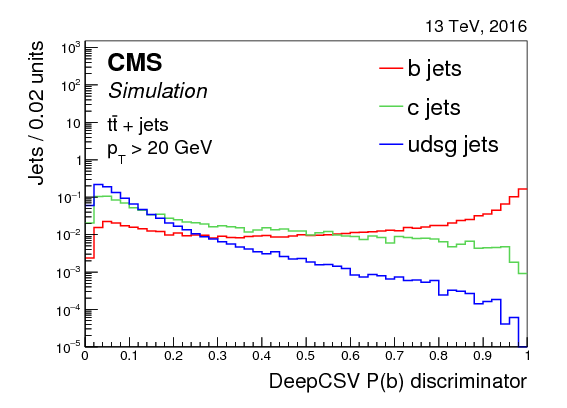
\includegraphics[width=0.45\textwidth]{Figures/PhysObj/deepCSV_b.png}}
			    \subfigure{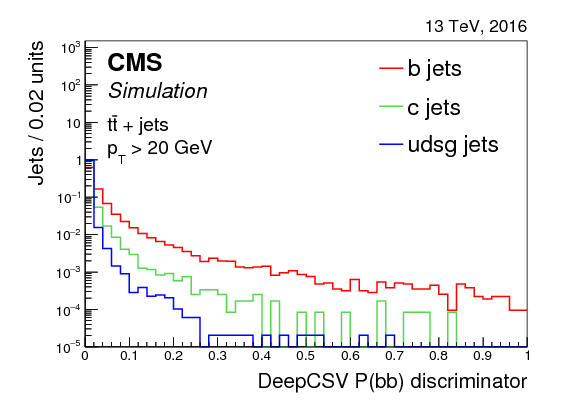
\includegraphics[width=0.45\textwidth]{Figures/PhysObj/deepCSV_bb.png}}\\
			\end{figure}
			\FloatBarrier
			\begin{figure}[H]
			\centering
			    \subfigure{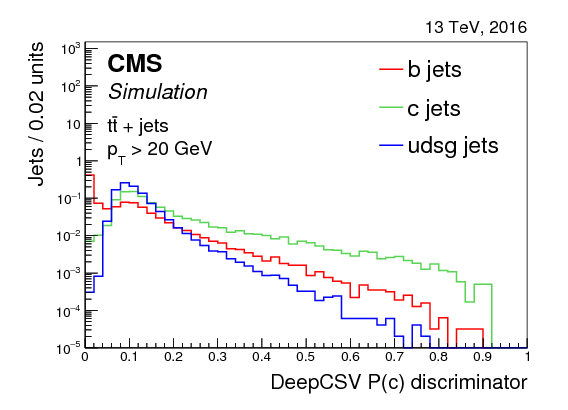
\includegraphics[width=0.45\textwidth]{Figures/PhysObj/deepCSV_c.png}}
			    \subfigure{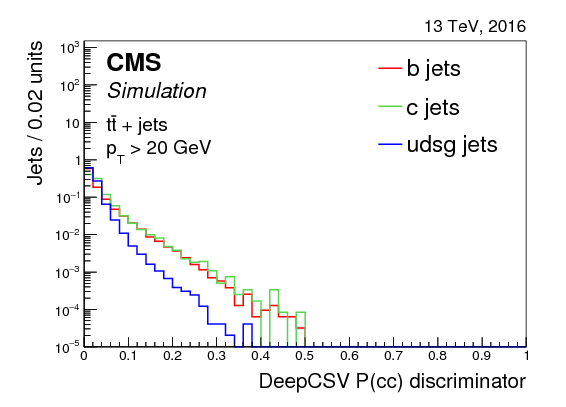
\includegraphics[width=0.45\textwidth]{Figures/PhysObj/deepCSV_cc.png}}\\
			\end{figure}
			\FloatBarrier
			\begin{figure}[H]
			\centering
			    \subfigure{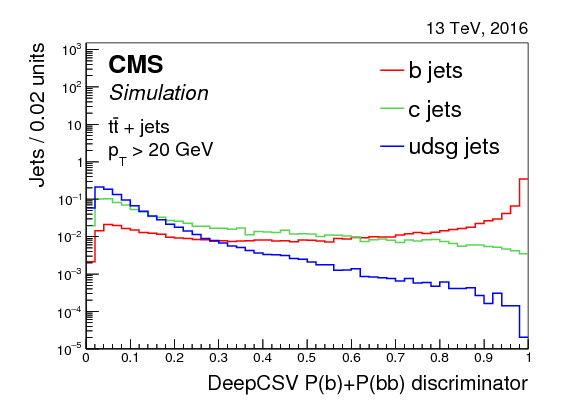
\includegraphics[width=0.65\textwidth]{Figures/PhysObj/deepCSV_b_bb.png}}\\
			\caption{Distribution of the DeepCSV P($b$), P($bb$), P($c$), P($cc$), P($b$) + P($bb$) discriminator values for jets of different flavors in $t\bar{t}$ events. Reference by \cite{CMS-BTV-16-002}}
			\label{PhysObj:fig:flavor_discr}
			\end{figure}
			\FloatBarrier

			The P($b$) + P($bb$) discriminator is used in the usual physics analysis with DeepCSV values. The DeepCSV b-tagging algorithm is used on the jets which passed the jet selection. In this analysis, there are two criteria would be used -- DeepCSV Medium(which is used in signal region) and DeepCSV Loose(which is used in control region). The criteria is applying thresholds on DeepCSV value, the thresholds which are from $\textbf{btagging}$ $\textbf{and}$ $\textbf{Vertex}$ $\textbf{Physics}$ $\textbf{Object}$ $\textbf{Group}$$\textbf{(BTV POG)}$'s\cite{btvpog_twiki} recommendation\cite{btagrecommendation_twiki} are shown below:

			\begin{itemize}
				\item DeepCSV Medium $\rightarrow$ Discriminator of DeepCSV is above 0.6321
				\item DeepCSV Loose $\rightarrow$ Discriminator of DeepCSV is within 0.2217-0.6321
			\label{PhysObj:itm:btag}
			\end{itemize}

	\subsection{Trigger}
	\label{ssec:PhysObj_trg}
		Trigger is the start of the physics event selection prrocess. There is a decision to retain a set of events which is included in and suitable to be used for specific analysis. There are 2 kinds of trigger in CMS trigger system. The following introduction are collected from reference \cite{Dasu:2000ge}, \cite{Cadamuro_2017}, \cite{Trocino_2014} . There are the $\textbf{Level}$ $\textbf{1}$ $\textbf{Trigger}$$\textbf{(L1T)}$ and the $\textbf{High}$ $\textbf{Level}$ $\textbf{Trigger}$$\textbf{(HLT)}$ system.

		
		The L1T is based on custom electronics. It is based on the identification of muons, electrons, photons, jets, and missing transverse energy. The L1T is selection about hardware components. It use the custom electronic boards to run event selection algorithms and to use the information from a subset of the CMS subdetectors, then make each decision in about $3.8\mu s$ and make output event rate to about 100kHz. To elaborate, there are global trigger system taking the information from local reigger system which collects the information from subdetector in every region in CMS. According to the decision and detemination, for instance, the whether the sum of some passed jets' $p_T$ are higher than given threshold , output events may be the worth-keeping events eventually. 

		\begin{figure}[H]
		\centering{}
			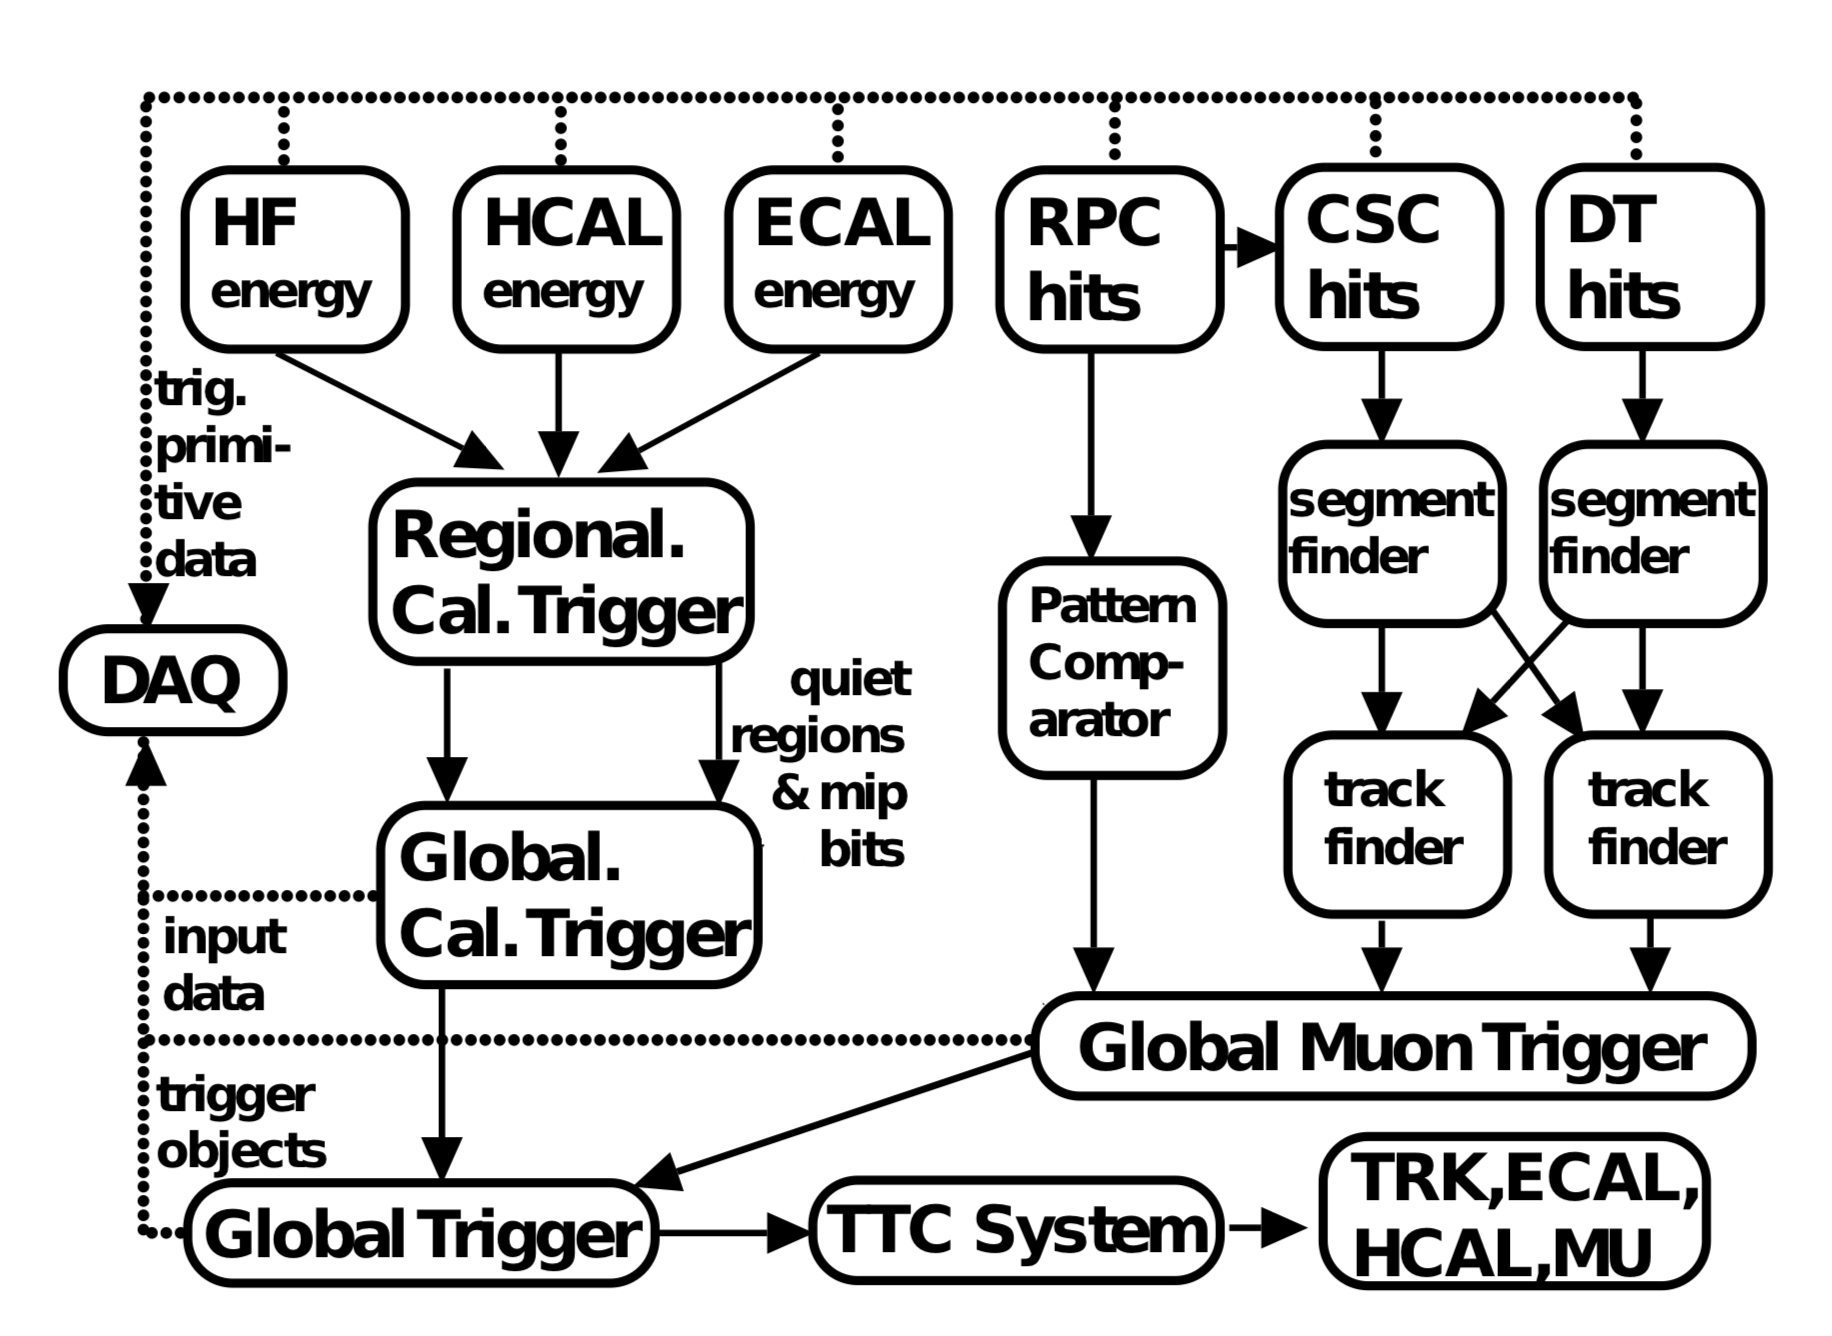
\includegraphics[width=0.85\textwidth]{Figures/PhysObj/L1T.png}\\
		\caption{Overview of the CMS L1 trigger system. \cite{Khachatryan:2016bia}}
		\label{PhysObj:fig:L1T}
		\end{figure}
		\FloatBarrier

		\begin{itemize}
			\item HF, HCAL, ECAL : data is originally from the forward, barrel hadronic calorimeters and the electromagnetic calorimeter,
			\item RCT, GCT : data is then processed first regionally and globally.
			\item PRC, CSC, DT : resistive plate chambers, cathode strip chambers, and drift tubes.
			\item GMT : nergy deposits (hits) from PRC, CSC and DT are processed either via a pattern comparator or via a system of segment- and track-finders and sent onwards to a global muon trigger (GMT). 
			\item GT : The information from the GCT and GMT is combined in a global trigger (GT), which makes the final trigger decision.
			\item MU, TTC : This decision is sent to the tracker (TRK), ECAL, HCAL or muon systems (MU) via the trigger, timing and control (TTC) system. 
			\item DAQ : the data acquisition system reads data from various subsystems for offline storage. 
			\item MIP : minimum-ionizing particle.
			\item Above are from overview of the CMS L1 trigger system. \cite{Khachatryan:2016bia}
			\label{PhysObj:itm:L1T}
		\end{itemize}

		The HLT relies upon commercial process, and it's software based. While keeping the output rate and CPU time under control, HLT must ensure a large acceptance for physics signals. The high level trigger access the whole readout data and do some complicated calculation on them. Spliting selected events into non-exclusive streams would be its work. The high level trrigger may reduce the L1T's output events rate to a sustainable level for physical annalysis and storage.
		





\FloatBarrier
